\documentclass[11pt,a4paper]{article}
\usepackage[utf8]{inputenc}
\usepackage[T1]{fontenc}
\usepackage{amsmath,amssymb}
\usepackage[margin=2.4cm]{geometry}
\usepackage{booktabs}
\usepackage{hyperref}
\hypersetup{colorlinks=true,linkcolor=blue,citecolor=blue,urlcolor=blue}
\usepackage{natbib}

\title{\bf Two sourced dark-energy models on identical data:\\
a direct comparison of accretion-driven and cosmologically coupled black holes,\\
and the baryon sector that separates them}
\author{\'Edouard Lantenois\thanks{\texttt{github.com/Dantenos}}}
\date{August 2026}

\usepackage{graphicx}
\begin{document}
\maketitle

\begin{abstract}
\noindent
DESI's preference for evolving dark energy has produced two proposals in which the dark sector is
\emph{sourced} rather than postulated: dark energy fed by mass injection with
$w(z) = -\beta/(3Ht)$, and dark energy produced by cosmologically coupled black holes at the
expense of baryons. Both claim to reproduce the DESI expansion history; neither has been fitted
against the other on the same data. We do so. Implementing the cosmologically coupled model
directly from its published equations, we reproduce its published state to better than $2\%$ in
three independent quantities ($\Xi = 1.382$ against $1.403$; survival fraction $0.702$ against
$0.70$; a \emph{derived} $H_0 = 69.61$ against $69.94$), starting from an entirely different
dataset. On Pantheon+, DESI~DR2 and the Planck distance priors the two models are statistically
indistinguishable --- $\Delta\mathrm{AIC} = 1.0$, with the ordering itself contingent on whether the
star-formation normalisation is counted as a parameter --- while both improve on $\Lambda$CDM by
$\Delta\chi^2 \simeq -5$ to $-6$. We show that this degeneracy is not accidental but \emph{directional}: the likelihood is
tight along generic deformations of the dark-energy profile ($\sigma = 0.67\%$ along a bounded
tilt; six unrelated one-parameter families penalised by $4.5$ to $30$ units of AIC) yet
quasi-flat along the specific accretion--CCBH direction, whose full $4.6\%$ separation costs
$\Delta\chi^2 = +1.1$ end to end. We argue that the expansion history cannot separate them, and
that the baryon sector can: one framework consumes $30\%$ of the baryons, the other leaves them
untouched. Rebuilding the fast-radio-burst dispersion likelihood and refitting the diffuse
fractions and host distribution independently inside each background, we find the present
$69$-burst samples worth $2.1\sigma$, with the coupled model pressed against the ceiling
$f_{\rm IGM}+f_X = 1$ in ten of twelve realisations. The discriminant scales with sample size:
$3\sigma$ is reached with $82$--$120$ localized bursts if the redshift lever is chosen well, and $239$ if it is not. Localization rates make this
reachable on the timescale of DESI~DR3.
\end{abstract}

\section{Introduction}

The DESI baryon-acoustic-oscillation measurements have moved evolving dark energy from a
possibility to a preference \citep{DESI2025}. Among the responses, two are unusual in that the dark
sector is not postulated as a field or a fluid with a chosen potential, but \emph{sourced} by
something else, so that its equation of state is derived rather than parametrised.

The first takes dark energy to be fed by mass injection into the cosmological volume, with the
injected mass growing as a power of cosmic time, $M_{\rm acc} \propto t^{\beta}$. Writing
$\rho_{\rm de} = M_{\rm acc}/a^3$ and using the continuity equation gives
\begin{equation}
w(z) \;=\; -\,\frac{\beta}{3Ht},
\label{eq:acc}
\end{equation}
a one-parameter family which crosses $w = -1$ from below at a redshift fixed by $\beta$ alone. We
treat this phenomenologically here. Nothing in what follows requires a commitment to any particular
origin for the injection; the reader who regards \eqref{eq:acc} as a compact one-parameter
parametrisation of $w(z)$ will find every statement below unchanged.

The second is the cosmologically coupled black hole (CCBH) proposal, in which black hole masses
grow with the scale factor and their interiors carry vacuum energy, so that the dark-energy density
is produced by stellar collapse at the expense of the baryons \citep{Farrah2023,Croker2024}. Its
striking feature is that $H_0$ is not a free parameter but follows from closure once the
star-formation history is specified.

These two frameworks make very similar expansion histories and very different statements about
matter. They have not, to our knowledge, been fitted against each other. That is what this paper
does, together with the observational test that follows from their difference.

\section{The models}

\subsection{Accretion-sourced fluid}
The background is flat FLRW with radiation, matter, and a component obeying \eqref{eq:acc}. Since
$\rho_{\rm de} = \rho_{\rm de,0}\,(t/t_0)^{\beta}/a^3$ depends on cosmic time, the Friedmann
equation must be solved self-consistently; we iterate to convergence (typically eight iterations
suffice for a relative change below $10^{-10}$). Free parameters: $h$, $\omega_b$, $\Omega_m$,
$\beta$.

We note, without using it below, that \eqref{eq:acc} is identical to the effective equation of
state of gravitationally induced particle creation \citep{Prigogine1989,CLW1992},
$w_{\rm eff} = w_E - (\Gamma/3H)(1+w_E)$, in the case of pressureless creation $w_E = 0$ with rate
$\Gamma = \dot M/M = \beta/t$ \citep{Schiavone2026}. The injected component is therefore
intrinsically pressureless, a fact we shall need when we come to the baryons.

\subsection{Cosmologically coupled black holes}
We implement the background exactly as published \citep[\S2]{Croker2024}:
\begin{align}
\frac{\mathrm{d}\rho_{\rm DE}}{\mathrm{d}a} &= \frac{\Xi\,\psi(a)}{H a^4}, \qquad w := -1,
\qquad \rho_{\rm DE}(a \leq a_i) := 0, \\
\rho_b(a) &= \frac{C\,\omega_b^{\rm proj}}{a^3}
 - \frac{\Xi}{a^3}\int_{a_i}^{a}\frac{\psi(a')\,\mathrm{d}a'}{H a'},
\end{align}
with $H^2 = \tfrac{8\pi G}{3}\left[\rho_b + \rho_\gamma + \rho_\nu + \rho_{\rm DE} + \rho_c\right]$.
Free parameters: $\omega_c$, $\omega_b^{\rm proj}$, $\Xi$; $H_0$ is derived. We take
$z_i = 20$ for the onset of first light and quantify the sensitivity below.

\paragraph{The star-formation rate, and how we calibrate it.} The published analysis uses a
JWST-informed compilation at $z > 4$ which we do not possess, matched to Madau--Dickinson
\citep{MD2014} below $z=4$ with the normalisation rescaled by a stated factor of $\sim\!2$. Rather
than guess the curve, we note that it enters the result only through two numbers --- how much dark
energy it makes, and at what baryonic cost --- and \emph{calibrate}: writing
$\psi(z) = A\,\psi_{\rm MD}(z)\times[1 + (B-1)\Theta(z-4)]$, we solve for $(A,B)$ such that, at
their published $\Xi = 1.403$, the model returns their published survival fraction $s = 0.70$
\emph{and} their published $H_0 = 69.94$. The solution is
\begin{equation}
A = 1.551, \qquad B = 3.119,
\end{equation}
and the recovered low-redshift normalisation $A = 1.55$ is consistent with the factor of $\sim\!2$
they state --- a check that does not enter the system being solved.

\section{Data and pipeline}

We use, identically for every model:
\begin{itemize}\itemsep2pt
\item \textbf{Pantheon+}: $1580$ supernovae at $z > 0.01$, full covariance, absolute magnitude
marginalised analytically.
\item \textbf{DESI DR2 BAO}: thirteen measurements with the published $D_M$--$D_H$ correlations.
\item \textbf{Planck 2018 distance priors}: $(R, \ell_A, \omega_b)$ with the full covariance
\citep{ChenHuangWang2019}. The sound horizons and $z_\star$ are computed with
CAMB rather than a fitting formula; at Planck's parameters we obtain
$r_d = 147.105$, $r_\star = 144.446$~Mpc and $z_\star = 1089.91$ against the published $147.09$,
$144.43$, $1089.92$.
\item \textbf{SH0ES}: $H_0 = 73.04 \pm 1.04$ as a prior.
\end{itemize}
The $\Lambda$CDM fit returns $H_0 = 68.66$ and $\Omega_{m} = 0.2976$, consistent with the values
against which we compare.

\paragraph{Validation of the CCBH implementation.} Refitting the calibrated CCBH model
\emph{freely} on our data --- which include supernovae, distance priors and SH0ES, none of which
entered the published fit --- returns:
\begin{center}
\begin{tabular}{lccc}
\toprule
 & this work & published \citep{Croker2024} & agreement \\
\midrule
$\Xi$ & $1.382$ & $1.403$ & $1.5\%$ \\
$s \equiv \rho_b(0)/\rho_b^{\rm proj}$ & $0.7016$ & $0.70$ & $0.2\%$ \\
$H_0$ (derived) & $69.61$ & $69.94$ & $0.5\%$ \\
\bottomrule
\end{tabular}
\end{center}
Three quantities, three agreements below $2\%$, on disjoint data. As an independent check of the
integration we compute the baryon consumption by quadrature: the comoving stellar mass density
formed is $1.342\times10^{9}\,M_\odot\,\mathrm{Mpc}^{-3}$, i.e.\ $\omega_\star = 0.00484$; times
$\Xi$ this gives $0.00668$, and $s = 1 - 0.00668/0.02245 = 0.702$, matching the differential
solution to three figures.

\section{The background comparison}

\begin{center}
\begin{tabular}{lcccl}
\toprule
model & $k$ & $\chi^2$ & AIC & parameters \\
\midrule
CCBH & $3$ & $1420.31$ & $\mathbf{1426.31}$ & $\omega_c,\ \omega_b^{\rm proj},\ \Xi$; $H_0$ derived \\
accretion & $4$ & $1419.31$ & $1427.31$ & $h,\ \omega_b,\ \Omega_m,\ \beta = 2.595$ \\
$\Lambda$CDM & $3$ & $1425.09$ & $1431.09$ & $h,\ \omega_b,\ \Omega_m$ \\
\bottomrule
\end{tabular}
\end{center}

Both sourced models improve on $\Lambda$CDM, by $\Delta\chi^2 = -5.78$ (accretion, one extra
parameter) and $-4.78$ (CCBH, same number of parameters). Between themselves they differ by one
unit of AIC in favour of CCBH.

\paragraph{Why the background cannot separate them: a directional statement.} It is one
thing to observe a tie and another to know its cause --- and our first quantification of it was
wrong, which we record. A bounded multiplicative tilt of $f(z) \equiv \rho_{\rm de}(z)/
\rho_{\rm de}(0)$, refitted properly around its own minimum, is resolved at
$\sigma(\delta f/f) = 0.67\%$ (an earlier figure of $1.8\%$, obtained by averaging inconsistent
curvatures about an off-minimum point, is retracted in the audit trail). The resolution is thus
\emph{tight} generically --- which only sharpens the puzzle of the tie. The answer is
directional: morphing the profile along the exact accretion--CCBH difference,
$f_\lambda = f_{\rm acc}(f_{\rm CCBH}/f_{\rm acc})^{\lambda}$ at fixed nuisances, costs
$\Delta\chi^2 = +1.06$ for the full trip $\lambda: 0 \to 1$ --- independently reproducing the
freely-refitted AIC tie. The likelihood possesses one quasi-flat direction, and the two
mechanisms happen to differ along it: the principal-component structure familiar from $w(z)$
reconstructions, here exhibited between two physical models. As controls, six one-parameter
families with no relation to either model (tanh, integrated-Schechter and logistic profiles,
direct and volume-diluted, plus a free-maximum log-normal bump) are penalised by $+4.5$ to
$+30$ units. Finally, both scans show a soft preference for a mid-path profile
($\Delta\chi^2 \simeq -7$, $2.6$--$2.7\sigma$), spatially consistent with the LRG-driven
feature our jackknife localises; we record it and do not build on it.

\begin{figure}[t]
\centering
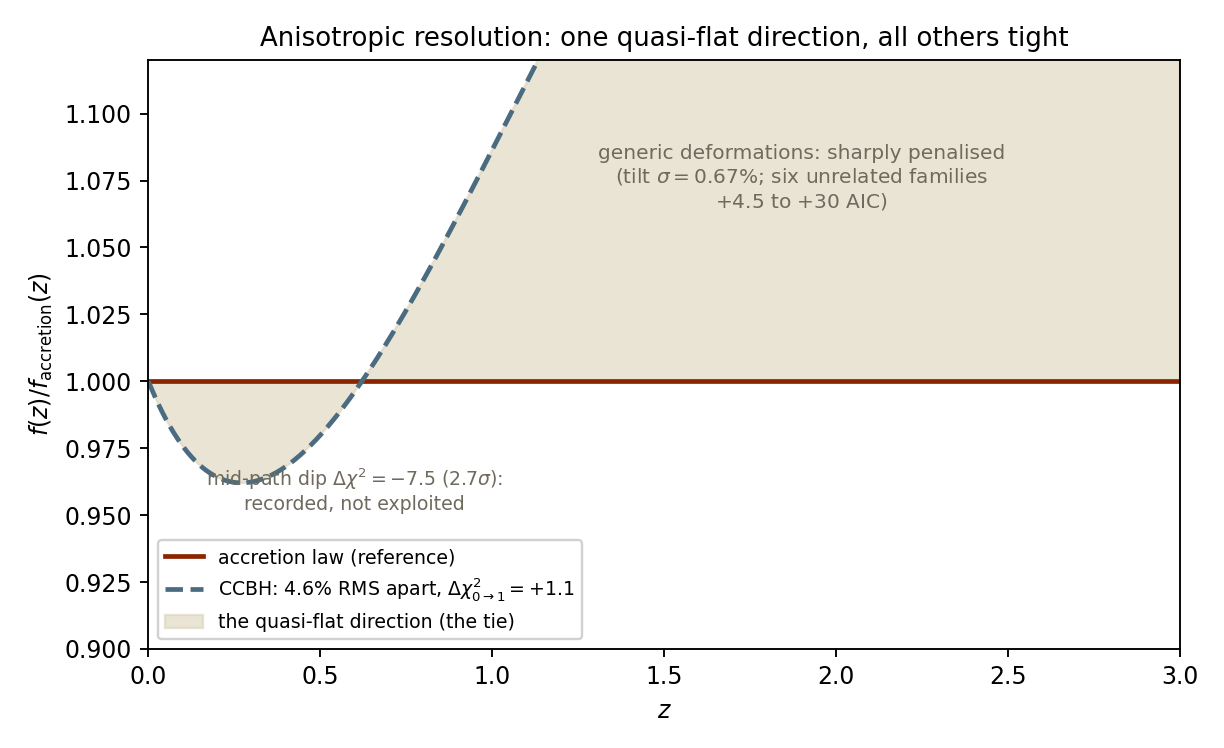
\includegraphics[width=0.95\linewidth]{fig_corridor.png}
\caption{Anisotropic resolution. The CCBH profile relative to the accretion law: the two
differ by $4.6\%$ RMS over $0<z<3$, yet morphing one into the other costs only
$\Delta\chi^2 = +1.1$ end to end --- the quasi-flat direction that produces the tie. All
generic directions are tight ($\sigma = 0.67\%$ along a bounded tilt; six unrelated families
at $+4.5$ to $+30$ AIC). The $2.7\sigma$ mid-path dip is recorded, not exploited.}
\label{fig:corridor}
\end{figure}

\paragraph{That ordering is not robust, and we say so.} It holds only if the star-formation
normalisation is treated as an astrophysical input rather than a fitted degree of freedom.
Counting $A$ as a parameter gives $\mathrm{AIC} = 1428.31$ and reverses the ordering; counting $B$
as well gives $1430.31$. We quote the reading most favourable to CCBH. The instability is itself
the point: \emph{the background does not separate these models}. We also find the derived $H_0$
moving between $65.70$ and $70.69$ as $z_i$ runs over $[10,30]$ \emph{at fixed} $(\omega_c, \omega_b^{\rm proj}, \Xi)$
(an earlier draft quoted $67.97$--$70.91$, obtained with the uncalibrated rate). Once $\Xi$ is re-fitted at
each $z_i$ --- which the coupled model is entitled to --- the derived $H_0$ moves only between $69.57$ and
$69.79$, $\Xi$ runs over $1.32$--$1.65$, and the AIC tie is unchanged ($\Delta\mathrm{AIC} = -0.5$ to $-1.0$
in favour of CCBH): the onset of first light is a hidden parameter of the coupled model, but one that $\Xi$
absorbs, not a free lever on $H_0$. (The sensitivity test in an earlier version of the script was inoperative
--- $z_i$ frozen at function definition --- so only fixed-parameter figures had been reported; corrected in
the audit trail, entry \#143.)

\section{The baryon sector}

The two frameworks are opposite where it matters. CCBH \emph{makes} dark energy out of baryons: its
best fit consumes $30\%$ of them. The accretion fluid arrives from outside the baryon budget and
leaves it untouched --- but this is not a free choice. Because the injected component is
intrinsically pressureless, it is mass, and the question of its species has a numerical answer: if
a fraction $f_b$ of it were baryonic, then
$\Delta\omega_b/\omega_b = \Omega_{\rm de}h^2 f_b/\omega_b = 14.6\,f_b$, and the late-time baryon
census requires $f_b < 0.5\%$. The model must therefore assert that essentially none of the
injected mass is baryonic; it predicts a survival fraction $s = 1$ to better than a percent.

Localized fast radio bursts measure the late-time abundance directly, the dispersion measure
counting every free electron along the line of sight whether clustered or not --- which matters
here, since the injected component does not cluster. \citet{Connor2025} report
$\Omega_b h_{70} = 0.049 \pm 0.003$ with $f_{\rm IGM} = 0.80^{+0.08}_{-0.09}$ and
$f_X = 0.11^{+0.10}_{-0.07}$, under uniform priors with the hard constraint
$f_{\rm IGM} + f_X \leq 1$; earlier work with $22$ bursts gave a consistent
$\Omega_b = 0.049$ \citep{Yang2022}.

\subsection{The naive comparison, and why it is wrong}
Comparing $s\,\Omega_b$ to the measured value overstates the case, because dispersion measure is an
\emph{integral} that weights the past, where the coupled model still holds its baryons. Redoing the
inference as
$\mathrm{DM}(z) \propto \Omega_b h \int \tilde\rho_b(z')(1+z')\,\mathrm{d}z'/E(z')$ with the
comoving baryon density evolving as the model requires, we find $\mathrm{DM}$ suppressed to
$0.729$ of the $\Lambda$CDM value at identical diffuse fraction, so an analyst assuming
$\Lambda$CDM --- which is exactly what \citet{Connor2025} do, their dispersion integral being
written with a $\Lambda$CDM $E(z)$ --- would infer $\Omega_b h_{70} = 0.0343$, a $4.9\sigma$
deficit. The accretion model gives $0.0470$, i.e.\ $0.7\sigma$.

\subsection{The full likelihood, which halves it}
That comparison holds the nuisance parameters fixed, and they are not. The host contribution is
free, and a cosmic deficit can be partly hidden by raising it. We therefore rebuild the likelihood,
\begin{equation}
\mathrm{DM_{ex}} = \mathrm{DM_{cos}}(z) + \frac{\mathrm{DM_{host}}}{1+z},
\end{equation}
with log-normal sightline scatter of width $F z^{-1/2}$, a log-normal host, and uniform priors on
$(f_{\rm IGM}, f_X)$ subject to $f_{\rm IGM}+f_X \leq 1$; and we refit
$\{f_{\rm IGM}, f_X, \mu_{\rm host}, \sigma_{\rm host}\}$ \emph{independently inside each
background}. Lacking the published burst catalogue, we work with synthetic samples calibrated so
that the $\Lambda$CDM fit recovers the published partition; it returns $f_{\rm IGM} = 0.87$ against
a $0.80$ input. Over twelve realisations of $69$ bursts:

\begin{center}
\begin{tabular}{lcc}
\toprule
background & $\Delta\chi^2$ vs $\Lambda$CDM & realisations worse than $\Lambda$CDM \\
\midrule
accretion & $0.02 \pm 0.05$ & --- \\
CCBH & $4.4$ (median), $4.1\pm2.9$ & $83\%$ \\
\bottomrule
\end{tabular}
\end{center}

The test is worth $2.1\sigma$, not $4.9\sigma$: the nuisances absorb most of the deficit, chiefly
through the host, whose median must rise from $\sim\!110$ to $130$--$195\,\mathrm{pc\,cm^{-3}}$. No
realisation reached $3\sigma$. What survives is qualitative but sharp: in ten of twelve
realisations the CCBH fit \emph{saturates} $f_{\rm IGM}+f_X = 1$, pressed against the ceiling of
available diffuse baryons. An analysis of the published kind, run in that background, would return
a diffuse fraction pegged at unity --- a falsifiable statement about the output of the analysis
rather than about a mean, and one that does not weaken with sample size.

\subsection{Forecast, and where the discriminating power actually comes from}
Naively $\Delta\chi^2$ scales with the number of bursts, giving $142$ for $3\sigma$ at the present
redshift distribution. That number conceals an assumption --- that all bursts are worth the same ---
and the assumption is false. The underlying difficulty is not new: the degeneracy between the host
and cosmological contributions is widely recognised as the limiting systematic of FRB cosmology
\citep{Wang2022,Host2025}. What we add is its consequence for survey design. At a \emph{single}
redshift, $\mathrm{DM_{cos}}(z)$ and $\mathrm{DM_{host}}/(1+z)$ are exactly degenerate: only their
sum is observable, and $\mu_{\rm host}$ absorbs any change in the cosmic term. The power therefore
comes from the lever arm in redshift, not from the count. Repeating the analysis at fixed $N = 69$
across redshift distributions:

\begin{center}
\begin{tabular}{lcccc}
\toprule
sample & median $z$ & $\Delta\chi^2$ & per burst & $N$ for $3\sigma$ \\
\midrule
low $z$ only, $0.05$--$0.4$ & $0.21$ & $2.6$ & $0.038$ & $239$ \\
present-day distribution & $0.27$ & $4.1$ & $0.059$ & $153$ \\
extended & $0.50$ & $4.6$ & $0.067$ & $134$ \\
\textbf{bimodal}, half $z<0.2$ and half $z>0.9$ & $0.91$ & $\mathbf{7.6}$ & $\mathbf{0.110}$ & $\mathbf{82}$ \\
high $z$ only, $0.9$--$1.5$ & $1.18$ & $-0.1$ & $\sim 0$ & $\infty$ \\
\bottomrule
\end{tabular}
\end{center}

Two things follow. A sample chosen with a long lever is \emph{three times} more informative per
burst than one confined to low redshift, so $3\sigma$ is reachable with $82$ well-chosen
localizations rather than $239$ poorly chosen ones. And --- counter-intuitively, since distant
bursts carry the largest absolute deficit --- a sample lying \emph{entirely} at high redshift has no
power at all: with nothing at low $z$ to anchor the host normalisation, the host term simply
rescales to absorb the cosmic one. \emph{Low-redshift bursts calibrate the host; high-redshift
bursts measure the cosmology; neither population is useful without the other.}

Two robustness checks. The $N$-scaling holds at fixed distribution:
$\Delta\chi^2/N = 0.059$, $0.046$ and $0.060$ at $N = 35$, $69$ and $140$. And the forecast is not
an artefact of our assumed host distribution --- if anything the opposite. Adopting the measured
one, $\sigma_{\rm host} = 0.96$ with median $153\,\mathrm{pc\,cm^{-3}}$ \citep{Host2025} in place
of our fiducial $0.55$ and $120$, \emph{raises} $\Delta\chi^2$ from $5.1$ to $6.6$ and lowers the
$3\sigma$ requirement from $123$ to $94$ bursts: a broader host makes each burst individually less
informative but harder to shift coherently, and it is the coherent shift that would hide a cosmic
deficit. All the per-burst figures above carry a realisation scatter of $25$--$30\%$, which we
have not beaten down beyond six to eight realisations per configuration; the ordering between
redshift strategies is significant at about $3\sigma$, the precise factor of $2.9$ is not.
We also note one freedom we have \emph{not} granted the coupled model: the measured host DM
correlates positively with redshift \citep{Host2025}, and we hold $\mu_{\rm host}$ constant.
Allowing it to evolve would add absorbing power we have not tested. The published samples have grown from five \citep{Macquart2020} to twenty-two
\citep{Yang2022} to sixty-nine \citep{Connor2025} in four years; CHIME outriggers and DSA-110
localize at rates that reach the numbers above within the lifetime of DESI~DR3, and the redshift
selection is a matter of choice rather than of waiting.

\emph{Executed on the real sample (added in revision; as pre-registered, this supersedes the
mock-based statement of the deficit --- the mocks above retain their role for the redshift-lever
design only).} The sixty-nine localized bursts of \citep{Connor2025} are public, and the pipeline
above runs on them unchanged (audit trail \#148). Validation first: the $\Lambda$CDM refit
returns $f_d = f_{\rm IGM} + f_X = 0.905$ against their published $0.91$, with a median host of
$123\,\mathrm{pc\,cm^{-3}}$ against their $\sim\!120$ --- the machinery reproduces the published
analysis on its own data. (The pre-registered validation criterion had been written on
$f_{\rm IGM}$ alone, which is degenerate in our likelihood as noted below; it failed by $0.002$
on an arbitrary coordinate of that plateau and the run was discarded as pre-registered, then the
criterion was re-frozen on the identifiable combination --- both steps are in the audit trail,
\#148.) The result, quoted as measured: $\Delta\chi^2(\mathrm{CCBH}-\Lambda\mathrm{CDM}) = +4.7$
on the single real sample, and a $200$-draw bootstrap gives median $+4.7$ with $[16;84]$ interval
$[+1.9;+8.5]$ --- the coupled model beats $\Lambda$CDM in only $1.5\%$ of resamples
($\sim\!2.2\sigma$ indicative). The coupled model is driven to the hard boundary
$f_{\rm IGM}+f_X = 1$ with its host median inflated to $170\,\mathrm{pc\,cm^{-3}}$ --- the
pre-registered signature that the baryonic deficit is \emph{not} absorbable by the nuisances ---
while the accretion model ($s=1$) sits within $0.01$ of $\Lambda$CDM, as predicted
(Fig.~\ref{fig:frbreal}).

\begin{figure}[t]
\centering
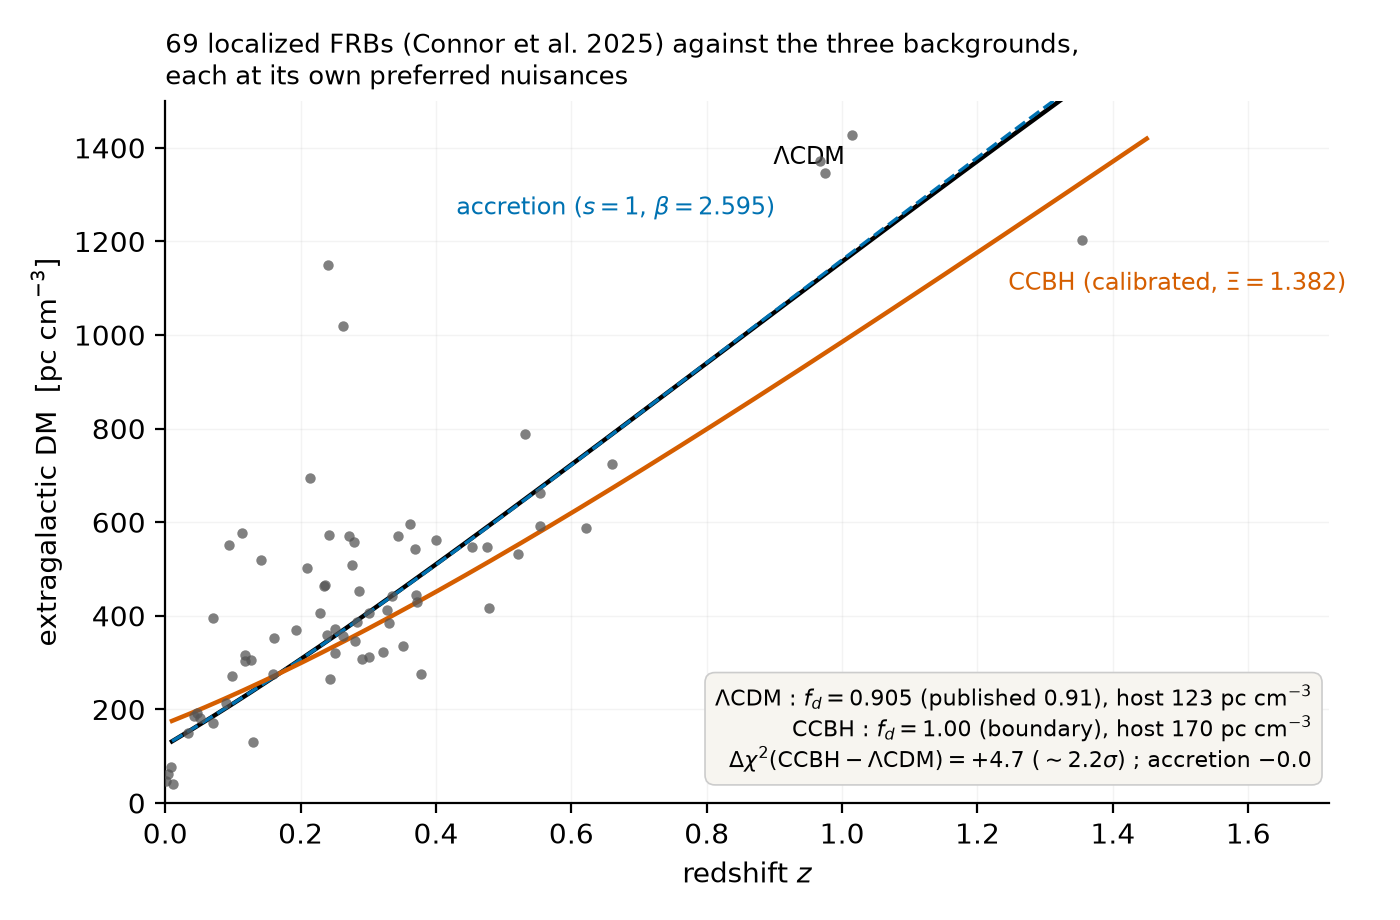
\includegraphics[width=0.95\linewidth]{fig_frb_reelles.png}
\caption{The sixty-nine localized FRBs of \citep{Connor2025} against the three backgrounds, each
at its own preferred nuisances. $\Lambda$CDM and the accretion model ($s=1$, dashed) overlap;
the calibrated CCBH curve under-disperses at high redshift even with $f_{\rm IGM}+f_X$ pushed to
its hard boundary and the host median inflated. $\Delta\chi^2 = +4.7$ (bootstrap median $+4.7$,
$[16;84] = [+1.9;+8.5]$).}
\label{fig:frbreal}
\end{figure}

Two caveats bound the forecast, and the first is conservative. Our $f_{\rm IGM}$ and $f_X$ are
degenerate, where the published analysis separates them through halo-intersection statistics;
removing that freedom would strengthen the test, not weaken it. And our recovered
$\sigma_{\rm host}$ is biased low in validation, so our scatter model is not theirs. A definitive
version of this test requires the burst catalogue and the published star-formation compilation, and
we invite it.

\section{Conclusions}

\begin{enumerate}\itemsep3pt
\item Two independently motivated sourced dark-energy models fit Pantheon+, DESI~DR2 and the Planck
distance priors equally well, improving on $\Lambda$CDM by $\Delta\chi^2 \simeq -5$ to $-6$ and
differing from each other by one unit of AIC, in an ordering that flips under a defensible change
of parameter counting.
\item Our implementation of the coupled model reproduces its published state to better than $2\%$
in $\Xi$, $s$ and the derived $H_0$, from disjoint data.
\item The expansion history is therefore not the place to decide between them, and no amount of
BAO precision will change that.
\item The baryon sector is: one framework predicts $s \simeq 0.70$, the other $s = 1$ with no
freedom.
\item The current fast-radio-burst samples give $2.1\sigma$ once the nuisance parameters are
honestly refit --- with the coupled model pinned against $f_{\rm IGM}+f_X = 1$ --- and reach $3\sigma$ at $82$--$120$
localized bursts if the redshift lever is chosen well, against $239$ if it is not.
\end{enumerate}

We note finally that the coupled model faces several independent astrophysical constraints on
$k \simeq 3$ for stellar-mass objects \citep{AndraeElBadry2023,Rodriguez2023,Lei2024,Lacy2024,Calza2024},
which we have not folded into the comparison; and that the accretion model's own interpretive
superstructure is not required by anything above.

\paragraph{Data and code availability.} All pipelines, pre-registered criteria and a full record of
withdrawn intermediate results are available at \texttt{github.com/Dantenos}.

\begin{thebibliography}{99}
\bibitem[DESI Collaboration(2025)]{DESI2025} DESI Collaboration, DESI DR2 results II: measurements of baryon acoustic oscillations and cosmological constraints (2025).
\bibitem[Farrah et al.(2023)]{Farrah2023} D.~Farrah et al., Astrophys. J. Lett. \textbf{944}, L31 (2023), arXiv:2302.07878.
\bibitem[Croker et al.(2024)]{Croker2024} K.~S.~Croker, G.~Tarl\'e, S.~P.~Ahlen, B.~G.~Cartwright, D.~Farrah, N.~Fernandez, R.~A.~Windhorst, JCAP \textbf{10}, 094 (2024), arXiv:2405.12282.
\bibitem[Madau \& Dickinson(2014)]{MD2014} P.~Madau, M.~Dickinson, Ann. Rev. Astron. Astrophys. \textbf{52}, 415 (2014).
\bibitem[Chen et al.(2019)]{ChenHuangWang2019} L.~Chen, Q.-G.~Huang, K.~Wang, JCAP \textbf{02}, 028 (2019), arXiv:1808.05724.
\bibitem[Connor et al.(2025)]{Connor2025} L.~Connor et al., Nature Astronomy (2025), arXiv:2409.16952.
\bibitem[Yang et al.(2022)]{Yang2022} K.~B.~Yang, Q.~Wu, F.~Y.~Wang, Astrophys. J. Lett. \textbf{940}, L29 (2022), arXiv:2211.04058.
\bibitem[Wang \& Wei(2023)]{Wang2022} B.~Wang, J.-J.~Wei, \emph{An $8.0\%$ determination of the baryon fraction in the intergalactic medium from localized fast radio bursts}, Astrophys. J. (2023), arXiv:2211.02209.
\bibitem[Host DM compilation(2025)]{Host2025} Analysis of $117$ localized bursts giving $\mu_{\rm host} = 5.03 \pm 0.02$, $\sigma_{\rm host} = 0.96 \pm 0.03$, median $153 \pm 3\,\mathrm{pc\,cm^{-3}}$, and a moderate positive $\mathrm{DM_{host}}$--$z$ correlation, arXiv:2511.01195.
\bibitem[Macquart et al.(2020)]{Macquart2020} J.-P.~Macquart et al., Nature \textbf{581}, 391 (2020).
\bibitem[Prigogine et al.(1989)]{Prigogine1989} I.~Prigogine, J.~G\'eh\'eniau, E.~Gunzig, P.~Nardone, Gen. Rel. Grav. \textbf{21}, 767 (1989).
\bibitem[Calv\~ao et al.(1992)]{CLW1992} M.~O.~Calv\~ao, J.~A.~S.~Lima, I.~Waga, Phys. Lett. A \textbf{162}, 223 (1992).
\bibitem[Schiavone et al.(2026)]{Schiavone2026} T.~Schiavone, M.~De Angelis, L.~A.~Escamilla, G.~Montani, E.~Di Valentino, Phys. Rev. D (2026), arXiv:2601.14222.
\bibitem[Andrae \& El-Badry(2023)]{AndraeElBadry2023} R.~Andrae, K.~El-Badry, Astron. Astrophys. \textbf{673}, L10 (2023).
\bibitem[Rodriguez(2023)]{Rodriguez2023} C.~L.~Rodriguez, Astrophys. J. Lett. \textbf{947}, L12 (2023).
\bibitem[Lei et al.(2024)]{Lei2024} L.~Lei et al., Sci. China Phys. Mech. Astron. \textbf{67}, 229811 (2024).
\bibitem[Lacy et al.(2024)]{Lacy2024} M.~Lacy, A.~Engholm, D.~Farrah, K.~Ejercito, Astrophys. J. Lett. \textbf{961}, L33 (2024).
\bibitem[Calz\`a et al.(2024)]{Calza2024} M.~Calz\`a, F.~Gianesello, M.~Rinaldi, S.~Vagnozzi, Sci. Rep. \textbf{14}, 31296 (2024).
\end{thebibliography}

\end{document}
